\documentclass[conference]{IEEEtran}
\usepackage{iftex}
\ifXeTeX
\usepackage{fontspec}
\setmainfont{Times New Roman}
\setsansfont{Arial}
\setmonofont{Courier New}
\else
\usepackage[T1]{fontenc}
\usepackage{mathptmx}
\usepackage{microtype}
\fi
\usepackage{amsmath,amssymb,array,url,graphicx,etoolbox,tikz}
\usetikzlibrary{positioning,arrows.meta}
\IfFileExists{booktabs.sty}{\usepackage{booktabs}}{\newcommand{\toprule}{\hline}\newcommand{\midrule}{\hline}\newcommand{\bottomrule}{\hline}}
\patchcmd{\abstract}{---}{: }{}{}
\patchcmd{\IEEEkeywords}{---}{: }{}{}
\newcolumntype{L}[1]{>{\raggedright\arraybackslash\hyphenpenalty=10000\exhyphenpenalty=10000}p{#1}}

% ======================================================================
% Revision of 17 November 2026. The \TBF placeholder block of the 14
% November revision is removed: every value below is copied from a recorded
% file, named in the text or in paper/README.md.
% Experiment 3 values: docs/evidence/lab-eval/20261117-main/RESULTS.md and
% summary.json. Parser re-run: docs/evidence/lab-eval/20261117-b-parser-rerun/
% summary.json. Set construction and freeze: docs/evidence/lab-eval-set-20261117/.
% E1 Windows replay: FINAL2/AUDIT.md, section 4. Deferrals: FINAL2/BLOCKERS.md.
% The local llama3.1:8b run of Experiment 3 was still running when this
% revision was built. Every line that must be filled from it carries the
% comment LLAMA-PENDING.
% ======================================================================
\newcommand{\PaperDate}{17 November 2026}
\newcommand{\Pending}{\emph{pending (run in progress)}}
% One sentence that only the student can confirm. It prints a visible marker.
\newcommand{\StudentConfirm}[1]{#1 \textbf{[student to confirm]}}

\title{LLM-Mediated Natural Language Controls for Short-Video Recommender Systems: An Offline Study of Controllability}
\author{\IEEEauthorblockN{Vibhor Malik}\IEEEauthorblockA{M.Sc. in Applied Computing, British Columbia Institute of Technology\\COMP 9500 Research Project. Supervisor: Borna Noureddin. \PaperDate}}
\begin{document}
\bstctlcite{paperBSTcontrol}
\maketitle
\thispagestyle{plain}\pagestyle{plain}
\begin{abstract}
This offline study asks how much a deterministic category control changes the exposure of a short-video feed and what it costs in next-item ranking quality, how reliably a language model interprets a request as a control, and whether control can go beyond fixed category identifiers. It separates interpretation by a model from a deterministic policy. In Experiment 1, target-category exposure is 79.2\% under a category policy against 11.6\% under one-item feedback, hard exclusion gives zero muted exposure, and NDCG@10 for boosts falls from 0.0301 to 0.0164; a Windows replay reproduces every reported metric but not the full-ranking hashes. A local Llama model parses 79 of 100 requests, below the 85\% target. In Experiment 2, with model-written references, Llama matches 76 of 100 and a rule parser 11, and conditional requests never succeed. The application now runs on real KuaiRec (865 users, 2,593 items) with a trained SASRec ranking and four language workflows over Chinese item text. Experiment 3 measures them on 40 new English and Chinese cases that an AI drafted and the student reviewed row by row (1,211 judgements, 24 corrections) and froze before any prediction. On 20 nonliteral requests, Claude Sonnet 5.5 and GPT-5 match the exact intended label profile on 17 and GPT-5 mini on 16; on 14 requests that should change nothing they abstain on 12, 10 and 7; on six new categories member F1 is 0.875 to 0.936. For 200 users, model controls raise target exposure from 0.6\% to 32.8--38.1\% (reviewed control 44.5\%) and lower NDCG@10. Intervals are wide, differences between models are not significant, and the local-model arm is incomplete. The study has no participants. % LLAMA-PENDING
\end{abstract}
\begin{IEEEkeywords}
controllable recommendation, natural-language interfaces, sequential recommendation, offline evaluation, human review
\end{IEEEkeywords}

\section{Introduction}
Item feedback communicates a reaction to one recommendation. A request such as ``show more of this category'' specifies a broader intervention. A profile carries a preference across requests. An explanation shows the information behind a recommendation. To compare these mechanisms, the interpretation of language must be separated from the enforcement of a control. Mozilla's 2022 audit of YouTube controls reported that Dislike prevented 12\% and Not interested 11\% of unwanted recommendations relative to its control group~\cite{ricks2022button}. That finding motivates the study; it is not a baseline.

The study asks three questions. First, how much does a deterministic category control change exposure on a frozen recommender, and what does it cost in next-item ranking quality? Second, how reliably does a language model interpret a request as such a control? Third, can language control go beyond fixed category identifiers, to existing category and tag names reached through indirect wording and to new categories, and how accurately do models do this against a human-reviewed reference?

The supervisor asked for three things: a manual category control with measured performance, a new category from natural language that feeds the filter, and indirect intent matched to existing categories and tags. Section~\ref{sec:app} describes one application on real KuaiRec data that serves all three, and Section~\ref{sec:e3} measures them. The model interprets or selects and never ranks; a fixed policy applies exactly what a person approved.

The study is offline and recruits no participants. It contributes two frozen experiments with their negative results, an integrated application, a bilingual evaluation set reviewed by a person and frozen before any prediction, a measurement of three hosted models on it, and a separation of four kinds of claim (Table~\ref{tab:claims}). It does not claim better accuracy or user satisfaction.

\section{Related Work}
\textbf{Language-based user models.} Radlinski et al. propose natural-language profiles for transparent and scrutable recommendation~\cite{radlinski2022profiles}. Balog et al. describe a set-based user model that can be shown to the user in natural language~\cite{balog2019transparent}. Ramos et al. let a language model write a profile and recommend from it, and report that edits change the recommendations~\cite{ramos2024transparent}. Other work studies editable and readable profiles~\cite{wozniak2025profiles,zhou2024language,mysore2023editable}, critiquing~\cite{chen2012critiquing} and language models that recommend from stated preferences or a conversation~\cite{sanner2023competitive,he2023zeroshot}. Harper et al. gave users a direct control over the popularity or recency of a list, and users rated the adjusted lists higher~\cite{harper2015control}. In most of these systems a language model or a learned profile takes part in ranking. Here the recommender is frozen; a model proposes only a command or an item set.

\textbf{Language models and control.} Lu et al. fine-tune a language model to follow recommendation instructions~\cite{lu2024aligning}. Dai et al. describe a re-ranking framework that accepts explicit attribute-based commands~\cite{dai2025token}. For short video, Niu et al. study a conversational control interface with a user study~\cite{niu2025chat}, and Fabbri et al. propose a transparent, controllable feed~\cite{fabbri2026feeding}. Both involve users; this study does not.

\textbf{Evidence and abstention.} Rashkin et al. define when a generated statement is attributable to an identified source~\cite{rashkin2023attribution}: a quotation can exist in a source and still not support a claim. Kamath et al. train a calibrator that decides when a model abstains~\cite{kamath2020selective}. The workflows here have no calibrated abstention; they abstain when the model reports ambiguity, no match or an unsupported operation.

\textbf{Evaluation.} Ji et al. show that splits that ignore the global timeline leak future interactions into training~\cite{ji2023leakage}. Zhang et al. argue that accuracy metrics do not directly measure alignment with stated preferences~\cite{zhang2026context}; their vision paper motivates the control measures used here but does not validate numerical bands. SASRec is the architectural basis of the recommender~\cite{kang2018sasrec}, and KuaiRec provides the data~\cite{gao2022kuairec}. The search for related work was not systematic, so the paper does not claim that any single element is new.

\section{Method}
\subsection{Data and information boundaries}
The processed cohort has 865 eligible users, 2,593 candidate items and 31 opaque category identifiers. The source is the fully observed small matrix of KuaiRec, with 1,411 users, 3,327 items and 4,676,570 interactions~\cite{gao2022kuairec}. A watch ratio (play duration divided by video duration~\cite{kuairecdocs}) above 2.0 is a derived positive-engagement proxy, not an observed like. Records without a timestamp are excluded. Shared chronological boundaries divide the source events into nominal 70\% training, 15\% request-history and 15\% evaluation windows. A user needs at least three training, two request-history and one evaluation positive.

Training uses only training sequences. Scoring receives training plus request history. Requests may use that history and the static categories, never the final behavioural labels. The first eligible final item supplies the relevance label, only after assignment and ranking. All catalogue items stay candidates, including items that a user has seen.

In Experiments 1 and 2, a category is an identifier such as \texttt{category\_12}, and synthetic requests are deterministic experimental assignments, not observations of what users wanted. KuaiRec also publishes a caption, cover text, topic tags and three levels of category names for each video~\cite{kuairecdocs}. Only the language controls of the application and Experiment 3 use them.

\subsection{Recommender and the five conditions}
The compact SASRec-style network (two self-attention blocks, one head, hidden size 32, maximum history 50, dropout 0.2) is trained with Adam (learning rate 0.001, batch size 64, gradient clipping 5.0) for 20 epochs with seeds 42, 43 and 44. It is an independently written variant, not a reproduction of published code, and its checkpoints stay fixed.

Five conditions use the same catalogue and the same frozen score vector. A is a simulated reaction to one historical item: the item is boosted or removed, with no language. B is A with explanations, which a model selects for display; its ranking must equal A. C is a free-text command and D one stored profile preference: a parser interprets, and one category policy applies. E combines C, D and explanations, merged once. The conditions do not identify the independent contribution of each mechanism. For each user, a hash selects one supported boost target and one mute target. The canonical wording of C and D was used during development, so that task is a consistency check, not a test of language generalization.

\subsection{Parsing, enforcement and explanations}
The language backend of Experiments 1 and 2 is local Llama 3.1 8B through Ollama, with constrained structured output and application validation. A transparent rule parser is a separate comparator; it never replaces a failed model call. An unknown category, an unsupported operation or a malformed output is an error that applies no control and stays in the denominator. Scores are normalized by each user's catalogue minimum and maximum. A category boost adds 0.25; a hard mute removes matching items, and no forbidden item is put back to fill a short list. Item identifiers break ties. An explanation selects one to three verbatim statements from verified item, category and history facts; it does not change the ranking of B.

\subsection{Metrics and statistical units}
At $K=10$, TCP@10 on a boost request and TCER@10 on a mute request are both $t/10$, where $t$ counts the first ten items that carry the requested category. The fill rate is reported so that an empty list cannot pass as a successful mute. HR@1 is one when the historical next item ranks first, and NDCG@10 is $1/\log_2(r+1)$ when that item appears at rank $r\leq10$. Both are next-item recovery proxies: a steering request can disagree with the historical next item.

In Experiment 1 the user is the unit: paired outcomes are averaged across requests and seeds within each user, so 865 users remain 865 units. Its primary contrasts are C, D and E against A for TCP and TCER, with two-sided Wilcoxon signed-rank tests (Pratt zeros), a Benjamini-Hochberg (BH) adjustment and user-bootstrap intervals (5,000 resamples). The proposal sets an 85\% target for exact parser accuracy, treats less than 70\% as degraded, and asks for top-1 hit rate ``within 10\%'' of the baseline without choosing an absolute or a relative margin. Failures stay in every denominator.

\subsection{Use of AI tools}\label{sec:ai}
AI tools took part in every stage. \emph{Code:} the student reports, as of 4 November 2026, that he supplied the project vision, used a language model to generate code, reviewed that code line by line and published it. That report does not cover later changes: the reviewed workflow, the integrated application of 16--17 November (the KuaiRec text join, the four workflows, the model providers), the measurement script and the metrics were produced with substantial AI assistance (Claude Code), and no line-by-line review by the student is claimed for them. The audit of 16--17 November and the Windows replay of Experiment 1 were run by Claude Opus 5.5 in Claude Code. \emph{Data and labels:} one authoring agent wrote the Experiment 1 parser bank. AI agents wrote the reference answers of the practice evaluation, the requests and both reference annotations of Experiment 2, and the requests and references of the 4 November study. In Experiment 2, the role names in the evidence files, among them the custodian name Vibhor, are names of AI roles, not of persons. The 40 cases and all reference judgements of Experiment 3 were drafted by Claude Opus 5.5; the student, Vibhor Malik, then reviewed every one of the 1,211 judgements himself. The English glosses of the item text are machine translations. \emph{Measured models:} the three hosted models of Experiment 3 are AI systems from two providers, one of them (Claude Sonnet 5.5) from the drafter's family. \emph{Demonstrations:} an AI session wrote the invented scenarios of 13 and 14 November, produced their model replies and made every review decision. \emph{Text:} an AI agent (Claude Opus 5.5) drafted this revision from the recorded evidence. \StudentConfirm{The student reviewed the text.} No AI tool is an author.

\section{Experiment 1: Category Control and Ranking}
Table~\ref{tab:e1} gives the frozen result. For boost requests, TCP@10 is 79.222\% under the category policy against 11.615\% under item feedback. For mute requests, TCER@10 is zero against 6.112\%. All lists are full. The direction follows from the policy: a category-wide boost reaches more items than a reaction to one item, and a hard mute gives zero by construction. C, D and E have identical rankings on equivalent canonical commands, and the rule parser gives the same rankings as Llama. The gain comes from the shared enforcement, not from the language model.

\begin{table}[t]\centering\footnotesize
\caption{Frozen Experiment 1 results, user means}\label{tab:e1}
\begin{tabular}{lrr}\toprule
Metric & A/B & C/D/E\\\midrule
Boost TCP@10 (\%) &11.615&79.222\\
Mute TCER@10 (\%) &6.112&0.000\\
Fill rate (\%) &100.000&100.000\\
Boost NDCG@10 &0.03012&0.01637\\
Mute NDCG@10 &0.03370&0.03526\\\bottomrule
\end{tabular}\end{table}

For C against A, the mean paired boost TCP difference is 67.607 points (95\% user-bootstrap interval 65.788 to 69.438), and the TCER difference is $-6.112$ points ($-7.056$ to $-5.241$). The adjusted Wilcoxon values are about $1.35\times10^{-142}$ and $1.05\times10^{-65}$.

\textbf{Negative results.} Boosting lowers NDCG@10 by 45.7\%; the post hoc paired difference is $-0.01375$ ($-0.02086$ to $-0.00655$). Mute requests move the other way, so one pooled value would hide two effects. The 85\% parser target is missed: Llama is correct on 79 of 100 broader synthetic requests (Wilson 95\% interval 70.02\% to 85.83\%) and the rule parser on 81. Llama is correct on all 70 supported positive, negative and reset cases, on 7 of 20 ambiguous or unsupported cases and on 2 of 10 adversarial cases; seven of its outputs are validation rejections and fourteen are valid but wrong. It parses all 120 canonical development inputs. One authoring agent wrote the 100 requests, and one test request differs from a development request only by a final period.

The non-inferiority reading is not useful. The baseline HR@1 of A is 0.25048\%. The absolute margin of 10 percentage points passes, but it would permit a complete loss of the baseline. The post hoc relative margin of 0.025 points does not pass: the simultaneous lower bound for C, D and E minus A is about $-0.077$ points. The backbone is weak: HR@1 per seed is 0.000\%, 0.347\% and 0.462\%, and a recent-popularity diagnostic reaches about 7.977\%. The ten generated explanation cards equal the template, so no explanation advantage was observed.

\textbf{Replay.} An earlier recomputation reproduced all 25,950 top-ten lists, but 2,009 full-ranking hashes and all 5,190 request-score hashes differed, and the original score vectors were not saved. On 16 November 2026 the frozen manifest was checked (288 of 288 files match) and the rule arm was replayed from the checkpoints on Windows 11 (Python 3.12.10, PyTorch 2.5.1+cpu, the frozen version) into a new folder. All 399 numeric values of the combined summary are identical to the frozen file, and every metric column is identical in all 25,950 request rows (8,650 per seed). The full-ranking hashes still differ in 605, 506 and 661 rows for seeds 42, 43 and 44, and the score hashes in all 1,730 records of each seed: raw scores differ below the top ten. The Llama arm was not replayed, because it needs the frozen parse cache; in the frozen records its rankings equal those of the rule arm. Every reported metric of Experiment 1 therefore reproduces; a bit-identical replay of the full rankings does not, and the cause is unresolved.

\textbf{Parser bank re-run (re-use, not new evidence).} On 17 November the same 100-case bank was sent again, unchanged, with the original prompt, schema and validator and no tuning (Table~\ref{tab:parser}). The bank was used in Experiment 1 and is exposed; every case uses the same 4 of the 31 opaque identifiers. Llama again scores 79 of 100, the frozen value. Under the strict primary score no model meets the 85\% target. The frozen prompt states ``Use strength 0.25 for boost, 1.0 for mute, 0.0 for reset/clarify''; GPT-5 and GPT-5 mini broke this rule on most reset and clarify cases, which the frozen validator rejects. A post hoc, format-lenient score ignores only the strength field on reset and clarify replies; it was computed on a second run that saved the raw replies, and it is secondary.

\begin{table}[t]\centering\scriptsize
\setlength{\tabcolsep}{2.6pt}
\caption{Parser bank re-run: RE-USE of the exposed 100-case bank of Experiment 1, not new evidence. Strict score of run~1 is primary (target 85\%; no model meets it); the format-lenient score is post hoc}\label{tab:parser}
\begin{tabular}{lrcrrrr}\toprule
Model & Strict 1 & Wilson 95\% & Op. err. & Clarify & Strict 2 & Lenient 2\\\midrule
Llama 3.1 8B & 79/100 & [0.700, 0.858] & 0 & 9/30 & not run & 79/100$^{a}$\\
Qwen2.5-Coder 7B & 74/100 & [0.646, 0.816] & 9 & 10/30 & not run & n/a$^{b}$\\
GPT-5 mini & 60/100 & [0.502, 0.691] & 36 & 0/30 & 60/100 & 95/100\\
GPT-5 & 60/100 & [0.502, 0.691] & 35 & 0/30 & 60/100 & 96/100\\\bottomrule
\end{tabular}\\[2pt]
\parbox{\columnwidth}{\scriptsize Local models through Ollama (temperature 0, seed 42); hosted models through the OpenAI API, low effort. Cost of run~1: USD 0.035 (GPT-5 mini), 0.188 (GPT-5), 0 (local). $^{a}$Recorded with zero errors. $^{b}$Raw replies not saved. Frozen Experiment 1: Llama 79/100, rules 81/100.}
\end{table}

\section{Exposed Practice Evaluation}
A practice run of 14 October 2026 used 100 questions and model-written reference answers that were already exposed. Validated whole-command agreement is 73 of 100 for Llama and 18 of 100 for rules. Llama has 24 rejections: 23 for a condition that the request did not ground and one for an invalid floor. User-averaged induced control success is 23.81\% for Llama, 8.40\% for rules and 3.92\% for item feedback, while NDCG@10 is 0.02461 against 0.03128. Exposed questions cannot support an unseen-test claim.

\textbf{Student response check.} On 20 October 2026 the student reports that he completed the worksheet of the 100 exposed practice questions himself, without the reference answers. His responses match 99 of the 100 model-written labels. This is a descriptive student-versus-model comparison, not agreement between two independent human annotators, and it is unresolved whether he had seen development summaries before. A parser-only check against his labels again gives 73 of 100 for Llama and 18 of 100 for rules.

\section{Experiment 2: Model-Written References}
Experiment 2 has its own protocol, frozen on 14 October 2026 before any request was written. A seeded plan of 100 slots balances four request classes, 25 each, over all 31 category identifiers: compound (boost one category and reduce another), graded (slight boost, strong reduction or exclusion), floor (reduce and keep at least one item) and conditional (boost only items that carry two categories). A model author wrote the wording. Two model annotators, AI roles of one model family in separate contexts, labelled the requests under a fixed rubric and agree on all 100 commands (Cohen's $\kappa=1.0$). This measures consistency between two contexts of one model family, not correctness, and the references are not human labels. A first annotation attempt was stopped before any comparison because both receipts lacked a required field; its labels are kept and were not used.

Experiment 2 has its own compound-command parsers and policy (adjustments of 0.10, 0.25 or 0.50, an optional floor of one item and a same-item condition). The unchanged local Llama 3.1 8B (Ollama 0.34.0, temperature 0, seed 42) and the rule parser each attempted every request once. The same 865 users, 2,593 items and three checkpoints supply matched item-feedback, rule, Llama and recency conditions. Induced success requires ten returned items, a class-specific category-count band and a positive rank-weighted movement of exposure in the requested direction (protocol: \url{docs/ai-reference-e2-protocol-2026-10-14.md}). Users are the units, and eleven one-sided Wilcoxon tests share one BH correction.

\textbf{Results.} Llama matches 76 of 100 references and the rule parser 11. By class, Llama matches 25, 24, 25 and 2 of the 25 compound, graded, floor and conditional references, and the rule parser 6, 5, 0 and 0. The other 24 Llama requests are 23 validation rejections of conditional requests with an ungrounded condition and one accepted command with a wrong floor. The rule parser returned a clarification for 89 requests.

\begin{table}[t]\centering\footnotesize
\caption{Experiment 2: ranking outcomes, user means. Success is induced control success}\label{tab:airank}
\begin{tabular}{lrrr}\toprule
Condition & Success (\%) & HR@1 (\%) & NDCG@10\\\midrule
Item feedback & 3.815 & 0.241 & 0.03184\\
Rules & 3.854 & 0.231 & 0.03097\\
Llama & 20.145 & 0.337 & 0.02580\\
Recency & 5.202 & 7.977 & 0.11866\\
\bottomrule
\end{tabular}\end{table}

Table~\ref{tab:airank} gives the ranking outcomes. The pooled Llama gain in induced success over item feedback is 16.3 percentage points (95\% interval 15.1 to 17.6), and over rules 16.3 points (15.2 to 17.4). Nine of the eleven tests are significant after correction; the two tests on conditional requests are not, since all differences are zero. Of 10,380 request-seed assignments, 987 are structurally infeasible and 5,586 have no directional opportunity; all stay in the denominator.

\textbf{Negative results.} Conditional requests have 0.000\% induced success in all four conditions, and Llama matches only 2 of 25 conditional references. NDCG@10 is 0.02580 for Llama against 0.03184 for item feedback (paired difference $-0.0060$, interval $-0.0084$ to $-0.0038$). HR@1 is 0.337\% against 0.241\%, a difference whose interval includes zero.

\section{The Integrated Application on KuaiRec}\label{sec:app}
Until 14 November the language controls ran only on invented scenarios of eight to ten items with a diagnostic scorer, while the five conditions ran on KuaiRec. One local application now serves both on the same processed KuaiRec data (865 users, 2,593 items, 31 opaque identifiers). The trained SASRec checkpoint of seed 42 scores every item for the chosen user from training plus request history, and the scores are min-max normalized. The study view serves A to E unchanged; because the processed categories are \texttt{category\_N} identifiers, C, D and E work there with the frozen rule parser.

\textbf{Item text.} The application joins the KuaiRec caption table to the processed items by video identifier: caption, manual cover text, topic tags and three levels of category names. The table covers all 2,593 items, 2,513 of them with a caption or cover text. The text is mostly Chinese. Each item can carry an English gloss, labelled as machine translation and given as a reading aid, never as source text. The model sees 467 label terms: all 266 category names and the 201 topic tags that at least three items carry (the other tags stay usable by hand).

\textbf{Policy.} A label is an opaque identifier, a category name, a tag or a new category that a person reviewed. \emph{Hide} removes the items that carry it, \emph{only} keeps them, and \emph{boost} or \emph{reduce} adds or subtracts 0.10, 0.25 or 0.40 (light, standard, strong) on the normalized score; the item identifier breaks ties. A preview changes nothing and shows the feed before and after; Apply accepts only a preview of the current state, and Undo restores the earlier state (Fig.~\ref{fig:stages}).

\begin{figure}[t]\centering
\newcommand{\stage}[2]{#1\vphantom{pl}\\[-1.5pt]{\fontsize{6}{7}\selectfont #2\vphantom{pl}}}
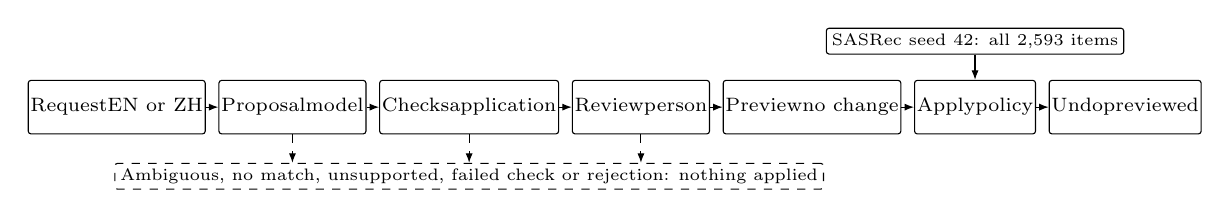
\begin{tikzpicture}[font=\scriptsize, node distance=1.6mm,
  st/.style={draw, rounded corners=1pt, align=center, minimum width=10.6mm, minimum height=6.8mm, inner sep=0.8pt},
  ar/.style={-{Latex[length=1.2mm]}}]
\node[st] (a) {\stage{Request}{EN or ZH}};
\node[st, right=of a] (b) {\stage{Proposal}{model}};
\node[st, right=of b] (c) {\stage{Checks}{application}};
\node[st, right=of c] (d) {\stage{Review}{person}};
\node[st, right=of d] (e) {\stage{Preview}{no change}};
\node[st, right=of e] (f) {\stage{Apply}{policy}};
\node[st, right=of f] (g) {\stage{Undo}{previewed}};
\foreach \x/\y in {a/b,b/c,c/d,d/e,e/f,f/g} \draw[ar] (\x)--(\y);
\node[draw, rounded corners=1pt, inner sep=2pt, above=3.2mm of f, font=\fontsize{6}{7}\selectfont] (s) {SASRec seed 42: all 2,593 items};
\draw[ar] (s.south) -- (f.north);
\node[draw, dashed, rounded corners=1pt, inner sep=2pt, below=3.6mm of c, font=\fontsize{6}{7}\selectfont] (h) {Ambiguous, no match, unsupported, failed check or rejection: nothing applied};
\draw[ar, dashed] (b.south) -- (b.south |- h.north);
\draw[ar, dashed] (c.south) -- (h.north);
\draw[ar, dashed] (d.south) -- (d.south |- h.north);
\end{tikzpicture}
\caption{Stages of a language control in the integrated application. The trained ranking is fixed; nothing changes before Apply.}\label{fig:stages}
\end{figure}

\textbf{Four workflows.} (1) \emph{Manual:} the person picks an existing label and an action; no model is called. (2) \emph{Request to existing labels:} one call receives the request, in English or Chinese and in any wording, and the 467 terms with their item counts and glosses, but no item text. It returns one control per preference, each with an action, a strength, a verbatim span of the request, exact term identifiers and a short relation, or the status ambiguous, no match or unsupported (quotas, time conditions and orderings). The application accepts only exact terms, and the members are all items that carry them. (3) \emph{New category:} a first call proposes a label (at most 60 characters) and a definition (at most 600) with quotations, and the person reviews it. Batched calls then classify every item of a scope (by default the user's top 40 items) as match, not match or unknown, each with an exact quotation. A separate check sees the item, the definition and the cited quotation, but never the verdict. An item is selected only if the verdict is match, the quotation is found in the named field and the check supports it. (4) \emph{New items:} for a new title and description, one call chooses existing categories, tags and a verdict for each reviewed new category, followed by the same check. A new item receives the median of the user's base scores and never enters the trained scorer.

\textbf{Providers.} The same workflow functions serve the application and the measurement script, so the measured behaviour is the shipped behaviour. Providers are an OpenAI-compatible endpoint, Ollama, the Anthropic Messages API, the Claude command-line program and a mock for tests. A test checks that the workflows contain no request-, label- or example-specific logic.

\section{Experiment 3: Language Controls on a Reviewed KuaiRec Set}\label{sec:e3}
\begin{table*}[t]\centering\footnotesize
\setlength{\tabcolsep}{3.4pt}
\caption{Experiment 3: requests to existing labels (NL, 20 cases) and requests that should change nothing (AB, 14 cases). 95\% intervals: Wilson for counts, bootstrap for F1}\label{tab:nlab}
\begin{tabular}{lccrrrrcrr|ccrr}\toprule
& \multicolumn{9}{c|}{NL: nonliteral request to existing KuaiRec labels} & \multicolumn{4}{c}{AB: should not propose}\\
& Exact & & Action & Label & Label & Label & & Missed & Unw. & Correct & & False & Status\\
Model & profile & 95\% CI & correct & prec. & recall & F1 & F1 95\% CI & req. & clar. & abstain & 95\% CI & accept. & match\\\midrule
Claude Sonnet 5.5 & 17/20 & [0.640, 0.948] & 95\% & 0.950 & 0.900 & 0.917 & [0.800, 1.000] & 4 & 1 & 12/14 & [0.601, 0.960] & 2 & 12\\
GPT-5 mini & 16/20 & [0.584, 0.919] & 95\% & 0.916 & 0.950 & 0.930 & [0.823, 0.997] & 2 & 1 & 7/14 & [0.268, 0.732] & 7 & 6\\
GPT-5 & 17/20 & [0.640, 0.948] & 100\% & 0.943 & 0.975 & 0.943 & [0.873, 1.000] & 1 & 0 & 10/14 & [0.454, 0.883] & 4 & 10\\
Llama 3.1 8B & \multicolumn{9}{c|}{\Pending} & \multicolumn{4}{c}{\Pending}\\ % LLAMA-PENDING
\bottomrule
\end{tabular}\end{table*}

\subsection{The evaluation set}
The set has 40 cases, 20 in English and 20 in Chinese. \emph{NL} (20; 10 per language) are nonliteral requests that express one preference indirectly, through a personal situation, slang, a metaphor or an example (a golden retriever arriving, a team knocked out of the playoffs, a brother on deployment). Each has one action (boost 7, reduce 6, hide 4, only 3), a \emph{required} label set that a careful annotator would select, an \emph{acceptable} set of defensible optional labels and three to six near-miss distractors; any other label counts as wrong. A script checked that the requests do not contain label names; only incidental words remain. \emph{NC} (6; 3 per language) describe concepts that KuaiRec has no single label for, such as first responders on duty or explicit money amounts; each has a reference label, an operational definition with inclusion and exclusion conditions, and member judgements over one shared pool of 150 items with text. Of the pool, 125 items were chosen on purpose as likely members and hard negatives, and 25 were drawn at random (seed 20261117). \emph{AB} (14; 7 per language) should not produce a control: ambiguous, hypothetical, negated or non-request statements, unsupported operations (an hourly quota, a weekday window, an ordering, a fixed ratio) and subjects with no match. Every request, description and definition was compared with 3,404 sentence segments of the earlier demonstration, parser and 4 November banks by character-trigram Jaccard similarity; the highest score was 0.222, with no exact or near-paraphrase overlap.

\textbf{Drafting, review and freeze.} Claude Opus 5.5 drafted all cases and 1,211 judgements (20 actions, 271 labels, 6 definitions, 900 memberships, 14 expected statuses). The student, Vibhor Malik, reviewed every row individually, not a sample, and judged the Chinese requests through the English gloss beside them. He agreed with 1,187 rows and corrected 24 (9 labels, 10 memberships, 2 definitions, 3 statuses). The rule of the tiered review protocol (stop at three or more wrong unflagged ``no'' rows) was met formally, with 3 of 796 such rows wrong; since every row was reviewed, all three were corrected. Nine items marked ``either'' are excluded from scoring for every model but stay in the pool. Three AB cases accept any abstaining status. The reviewed set was hashed (SHA-256 \texttt{d4af21e6ed311448\ldots}) and committed at 02:27:25 UTC on 17 November 2026, before any measured prediction; the first model run started at 02:28:10 UTC. No prompt, threshold or code that affects predictions was changed after the freeze; the only later change is an operational output cap for the local run (Section~\ref{sec:limits}).

\subsection{Models and procedure}
Claude Sonnet 5.5 (through the Claude command-line program), GPT-5 and GPT-5 mini (through the OpenAI API) ran at low effort. Each case was sent once through the application's own functions, with no retry after a wrong answer; every failure is kept. NL and AB cases use workflow~(2). NC cases use the classification and check of workflow~(3) with the \emph{reference} label and definition, so every model classifies the same 150 items under the same definition; the definition step itself is not measured. The local Llama 3.1 8B run was in progress when this revision was built. % LLAMA-PENDING
Using hosted frontier models is a declared departure from the proposal, which named local models only.

\subsection{Metrics}
\emph{NL:} with the selected label set $S$, required set $R$ and acceptable set $A$, a case is an \emph{exact intended profile} when the status is ``propose'', every control has the reference action and $R\subseteq S\subseteq R\cup A$. Label precision is $|S\cap(R\cup A)|/|S|$ and recall $|S\cap R|/|R|$; a missed required label is a retrieval miss. \emph{AB:} correct abstention means no applicable control; a false acceptance is any applicable control. \emph{NC:} member precision, recall and F1 of the selected items against the reference members, and the F1 of the raw verdicts. Proportions have Wilson intervals; means have percentile bootstrap intervals over cases (5,000 resamples, seed 2026).

\emph{Downstream:} 200 users with an evaluation item are sampled (seed 2026) and ranked by the seed-42 checkpoint. For each NL and NC case the target set is the items that carry the required labels (NL) or the scored reference members (NC). Three controls are compared: none, the reviewed reference control, and each model's control (an NC selection is applied as a boost). TCP@10 averages the share of the top ten in the target set over the 16 boost and only cases, TCER@10 over the 10 hide and reduce cases; NDCG@10 and HR@1 average over all 26 cases. HR@1 non-inferiority uses the bootstrap lower bound of the mean per-case difference from no control, against a relative margin of 10\% of the uncontrolled HR@1 and an absolute margin of 0.10. Fidelity compares each model's TCP@10 with that of the reference control per case (Wilcoxon, BH). Between models, an exact McNemar test compares per-case success (exact profile for NL, abstention for AB, member F1 $\geq0.8$ for NC) and a Wilcoxon test (Pratt) compares per-case scores (label F1, abstention, member F1), with BH across the three pairs ($\alpha=0.05$).

\subsection{Results}\label{sec:e3res}
\textbf{Requests to existing labels (Table~\ref{tab:nlab}).} Claude Sonnet 5.5 and GPT-5 match the exact intended profile on 17 of 20 requests and GPT-5 mini on 16; label F1 is 0.917, 0.943 and 0.930. GPT-5 chose the reference action in every case and missed one required label; Claude has the highest precision and missed four. The intervals overlap almost completely.

\textbf{Requests that should change nothing.} Claude abstains correctly on 12 of 14, GPT-5 on 10 and GPT-5 mini on 7. GPT-5 mini proposed a control for half of these requests. In the application a false acceptance reaches the reviewer as a proposal, so it is the main risk of a workflow without review.

\begin{table}[t]\centering\scriptsize
\setlength{\tabcolsep}{2.8pt}
\caption{Experiment 3: new-category membership (NC, 6 cases, shared pool of 150 KuaiRec items, reference definitions)}\label{tab:nc}
\begin{tabular}{lrrrcrr}\toprule
Model & Prec. & Rec. & F1 & F1 95\% CI & Raw F1 & Missed\\\midrule
Claude Sonnet 5.5 & 1.000 & 0.793 & 0.875 & [0.791, 0.959] & 0.970 & 21\\
GPT-5 mini & 0.942 & 0.934 & 0.936 & [0.887, 0.982] & 0.962 & 6\\
GPT-5 & 0.958 & 0.894 & 0.918 & [0.851, 0.976] & 0.953 & 11\\
Llama 3.1 8B & \multicolumn{6}{c}{\Pending}\\ % LLAMA-PENDING
\bottomrule
\end{tabular}\\[2pt]
\parbox{\columnwidth}{\scriptsize Selected: verdict match, quotation found in the item and the separate check supports it. Raw F1: classifier verdicts alone.}
\end{table}

\textbf{New categories (Table~\ref{tab:nc}).} Member F1 is 0.875 for Claude, 0.936 for GPT-5 mini and 0.918 for GPT-5. Claude selected no wrong member but missed 21 reference members. Its raw-verdict F1 is 0.970, so the quotation and evidence checks removed members that its classification had found; the checks trade recall for precision.

\begin{table}[t]\centering\footnotesize
\setlength{\tabcolsep}{4pt}
\caption{Experiment 3: downstream effect on the trained SASRec ranking (200 sampled users). TCP/TCER count the reference target set}\label{tab:down}
\begin{tabular}{lrrrr}\toprule
Control & TCP@10 & TCER@10 & NDCG@10 & HR@1\\\midrule
None & 0.0063 & 0.0118 & 0.0242 & 0.0050\\
Reviewed reference & 0.4447 & 0.0000 & 0.0160 & 0.0058\\
Claude Sonnet 5.5 & 0.3583 & 0.0000 & 0.0173 & 0.0042\\
GPT-5 & 0.3810 & 0.0000 & 0.0184 & 0.0056\\
GPT-5 mini & 0.3282 & 0.0000 & 0.0175 & 0.0044\\
Llama 3.1 8B & \multicolumn{4}{c}{\Pending}\\ % LLAMA-PENDING
\bottomrule
\end{tabular}\\[2pt]
\parbox{\columnwidth}{\scriptsize TCP@10: 16 boost/only cases; TCER@10: 10 hide/reduce cases; NDCG@10 and HR@1: all 26 NL and NC cases.}
\end{table}

\textbf{Downstream (Table~\ref{tab:down}).} The reviewed reference control raises TCP@10 from 0.0063 to 0.4447, and the model controls reach 0.3282 to 0.3810. Each model control stays below the reference control: the mean per-case differences are $-0.0864$ (Claude), $-0.0637$ (GPT-5) and $-0.1165$ (GPT-5 mini), with BH-adjusted Wilcoxon $p$ of 0.0054, 0.0050 and 0.0050 over 16 cases. Every control brings TCER@10 from 0.0118 to zero. NDCG@10 falls from 0.0242 to between 0.0160 and 0.0184, as in Experiments 1 and 2.

\textbf{Non-inferiority.} The uncontrolled HR@1 is 0.0050, one hit in 200 users, so the relative margin of 10\% is 0.0005. Against no control, the mean per-case HR@1 difference is $-0.0008$ for Claude, $0.0006$ for GPT-5 and $-0.0006$ for GPT-5 mini, with bootstrap lower bounds of $-0.0023$, $-0.0023$ and $-0.0021$; the mean NDCG@10 differences are $-0.0068$, $-0.0057$ and $-0.0066$. No model is non-inferior under the relative margin, and every model is under the absolute margin of 0.10, which is uninformative at this base rate. Llama 3.1 8B: \Pending. % LLAMA-PENDING

\textbf{Between models.} Over all 40 cases, Claude succeeds on 33, GPT-5 on 32 and GPT-5 mini on 29. No pairwise difference is significant: the BH-adjusted McNemar $p$ is 1.000 for Claude against GPT-5 and 0.762 for each comparison with GPT-5 mini, and the BH-adjusted Wilcoxon $p$ on per-case scores is 0.571, 0.269 and 0.269. With 40 cases the study cannot rank these models.

\textbf{Cost and failures.} The 411 calls (136, 137 and 138) had no call or case error. Median latency per call is 6.6\,s for Claude, 12.5\,s for GPT-5 and 11.7\,s for GPT-5 mini (90th percentile 7.8, 23.9 and 16.7\,s). Cost is USD 5.86 for Claude, as reported by the command-line program, and USD 2.39 and 0.47 for GPT-5 and GPT-5 mini at list price; local models cost no fee (electricity not counted). Llama 3.1 8B: \Pending. % LLAMA-PENDING

\section{Earlier Evidence for the Language Workflows}
This evidence predates the integrated application and Experiment 3, and none of it measures accuracy on KuaiRec text.

\textbf{Synthetic-language study of 4 November 2026.} It evaluated an earlier pipeline, the reviewed topic profile, with a local Qwen2.5-Coder 7B Instruct model (Ollama 0.34.0). The requests quoted literal Chinese source phrases, so the study tests control of a named source scope, not indirect wording. An AI author wrote 100 supported and 20 ambiguous or unsupported requests, and a second AI role reviewed the locked references. The pipeline matched the complete intended profile on 48 of 100 supported requests and clarified correctly on 19 of 20 diagnostic requests. The 120 invocations gave 49 ready proposals, 61 clarifications, five grounding errors and five parser or schema rejections. By stratum, the correct counts are 11, 7 and 8 of 20 for single boosts, reductions and exclusions, 15 of 20 for two-topic requests, 1 of 10 for profile replacements and 6 of 10 for single subjects with context. This is a negative finding for autonomous use. On 72 score vectors of 24 users and three seeds, the intended profile changed top-ten exposure by 5.3579 percentage points and the model-proposed profile by 2.9292 points; HR@1 and NDCG@10 are 2.33\% and 0.0611 for the intended profile and 2.29\% and 0.0617 for the model-proposed profile, against 2.54\% and 0.0650 for the initial profile. These are descriptive averages with no intervals.

\textbf{Development records.} A frozen twelve-request study of 5 November gave no approved application: new category 0 of 4 supported and 1 of 2 diagnostic requests; indirect request 0 of 4 and 0 of 2. The indirect cases stopped at a validation rule for the strength of an exclusion, a format failure rather than a measured semantic accuracy of zero. Across 14 retained development invocations on indirect requests, no local model produced an approvable item set. In the first frozen run of the staged workflow (0 of 2 applied), a local model proposed a definition whose valid quotations did not contain the claimed property, and the AI reviewer rejected it. In a standalone batch of six invented cases, a Claude model matched 6 of 6 tasks while a local Llama model and a later Qwen run failed strict JSON validation; that batch used different transports and is not a comparison.

\textbf{Demonstration runs on invented items.} On 13 November seven runs with real model output were recorded in a scripted browser on two invented scenarios of eight items; six completed, and the manual control, the new category and a request matched to descriptions each went through preview, Apply and Undo. On 14 November every method completed on revision \texttt{ff92666} (13 model calls, 321 of 321 scripted checks passed, 19 review decisions). In both, sub-agents of one AI session produced the replies and an AI operator made every review decision; the declared model was not attested, and the sub-agents were probably not blind to the intended answers. They show that the steps execute, not accuracy.

\section{Supported Claims, Limits and Reproducibility}\label{sec:limits}
Table~\ref{tab:claims} separates four kinds of claim. Evidence for one kind does not transfer to another.

\begin{table}[t]\centering\footnotesize
\caption{Four kinds of claim and the evidence for each}\label{tab:claims}
\setlength{\tabcolsep}{4pt}
\begin{tabular}{L{1.5cm}L{3.95cm}L{2.4cm}}\toprule
Claim&Evidence that exists&What is missing\\\midrule
The filter applies the approved set&Enforcement in Experiments 1 to 3; Experiment 1 metrics replayed on Windows; software and browser tests&A bit-identical replay of the full rankings\\
The interpretation is correct&Exp.~1: 79/100 (authored labels). Exp.~2: 76/100 and 4 Nov: 48/100 (model-written references). Exp.~3, AI-drafted and human-reviewed: NL exact 16--17/20, AB 7--12/14, NC F1 0.875--0.936&Independently written human references; larger samples; the local-model arm; natural requests\\
Ranking quality is kept&Not kept: NDCG@10 falls in Experiments 1, 2 and 3; relative HR@1 non-inferiority fails&A meaningful margin; a stronger backbone\\
People can use it and benefit&None&A user study\\\bottomrule
\end{tabular}\end{table}

\textbf{Reference and bias.} The Experiment 3 reference was drafted by an AI (Claude Opus 5.5) and reviewed, not written, by a person; a reviewer who reads a draft can anchor on it. Claude is both the drafter's family and a measured model (Claude Sonnet 5.5), which can favour Claude-family readings, for example in the required and acceptable sets; Claude's lead on AB cases should be read with this in mind. The Chinese requests were judged through an English machine-translation gloss, not by a reader of Chinese.

\textbf{Sample size.} With 20, 14 and 6 cases per group, the intervals are wide (exact profile 0.58 to 0.95) and no pairwise difference between models is significant. The set is now exposed and cannot serve again as an unseen test. HR@1 has a base rate of about 0.5\% on the sampled users, so the relative 10\% margin fails for every model while the absolute margin passes trivially. The downstream measure applies a prediction that mixes actions with a single action, and NC cases use the reference definition, so the definition step of workflow~(3) is not measured.

\textbf{Models not measured.} The local Llama 3.1 8B run of Experiment 3 is in progress; its first attempt was aborted by runaway generation, and the run was restarted from scratch with an operational cap of 2,048 output tokens (prompts and scoring unchanged). % LLAMA-PENDING
Gemma4 31B was not run: at 19\,GB it does not fit the 8\,GB GPU and 31.7\,GB RAM at the required 32k context. The Experiment 3 run of Qwen2.5-Coder 7B is deferred; only its parser re-run is complete. The Anthropic API route was not run live; Claude was measured only through the command-line program. Frontier models are a declared departure from the proposal's local-model-only design.

\textbf{Construct and external validity.} There is no user study: the work observes no real steering intention and measures no comprehension or satisfaction. The requests are written for the study, the next-item label is a historical proxy, and KuaiRec's platform, period and filtered cohort limit generalization. The backbone is weak and untuned. The earlier references of the practice evaluation, of Experiment 2 and of the 4 November study were written by models, and every bank that has been used once is exposed.

\textbf{Reproducibility.} The protocols, compact evidence files and the application are in the repository \url{https://github.com/vibhormalik95-hue/FP}. Experiment 3 summaries, per-case scores without item text and the frozen set hashes are under \url{docs/evidence/lab-eval/} and \url{docs/evidence/lab-eval-set-20261117/}; the review files contain KuaiRec item text and stay private. A separate research archive holds complete cases, model responses, ranking records and checkpoints. The Experiment 1 result files are not public, and the values of the twelve-request study, the development invocations and the student check are copied from earlier papers. A different inference runtime or a hosted model update may change model outputs.

\section{Conclusion}
A deterministic category policy changes exposure strongly and predictably, and it lowers next-item ranking quality for boosts; on a Windows replay all its reported metrics reproduce. On canonical requests it shows no advantage of a language model over rules. On fresh synthetic requests with model-written references, a local model compiles compound, graded and floor requests far more often than a rule parser and fails on conditional requests. The parser target of the proposal was missed, and useful non-inferiority was not established.

The application now serves the five conditions and four language workflows on real KuaiRec data with the trained ranking, and it answers the supervisor's three requests: a manual control, new categories that feed the filter and indirect requests matched to existing labels. On a bilingual set that a person reviewed row by row and froze before any prediction, three hosted models match the exact intended label profile on 16 or 17 of 20 nonliteral requests, abstain on 7 to 12 of 14 requests that should change nothing, and select new-category members with F1 from 0.875 to 0.936. Their controls move exposure toward the reviewed target but less far than the reviewed control, and NDCG@10 falls. The sample is small, the reference was AI-drafted, one measured model shares the drafter's family, and the local-model arm is incomplete. A larger set written independently by people, the local models, a stronger backbone and a user study are the next steps. % LLAMA-PENDING

\bibliographystyle{IEEEtran}
\bibliography{references-2026-11-14}
\end{document}
